\chapter{矢量}
矢量是多维空间的数字化体现,虽然看不到四维空间,但是我们就是可以操作四维矢量

\section*{学习目标}
\begin{todolist}
 \item 识别并使用矢量的标记
 \item 计算矢量的加减法以及数乘,并与之几何关系对应
 \item 求算矢量的模
 \item 能够利用单位矢量(方向矢量),位移矢量和位置矢量解决问题
 \item 理解三维空间当中直线的矢量标记形式 $\mathbf{r}=\mathbf{a}+\lambda\mathbf{b}$,并解释几何意义
 \item 根据已知信息求算空间当中的直线
 \item 判断空间当中的两条直线的位置关系,包括平行,相交,或者异面
 \item 求算两条相交的空间直线的交点
 \item 求算垂足以及空间内点到直线的距离
 \item 掌握两个矢量的点乘,并且能够使用矢量的点积解决立体几何问题
\end{todolist}
\clearpage

\section{矢量的相关概念和基本运算}
\begin{definition}
Vectors have both \textbf{Magnitude} and \textbf{Direction}.
\end{definition}
表示矢量的可以通过图像的方式,绘制成一个有方向的线段,其长度为该矢量的大小,方向用箭头表示。符号可以计作$\vec{a}$或者$\overrightarrow{OA}$
如下图所示:
\begin{figure}[H]
\centering
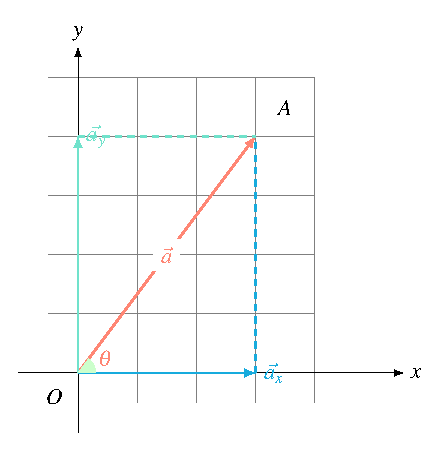
\includegraphics[width=0.3\textwidth]{vector}
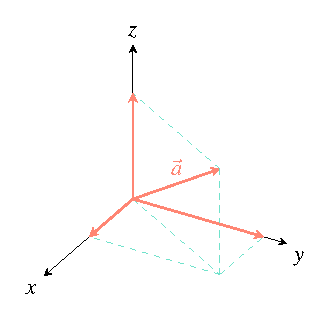
\includegraphics[width=0.3\textwidth]{3dvector}
\label{fig:vectors}
\caption{平面矢量的表示和正交分解}
\end{figure}

\subsection*{矢量的数乘}
如果$\vec{a}$代表一个矢量,那么$k\cdot \vec{a}$被称之为数值$k$乘以矢量$\vec{a}$。其意义是将矢量$\vec{a}$变成$k$倍。如果$k>0$,结果的矢量和$\vec{a}$的方向是一致的;如果$k<0$,结果的矢量和$\vec{a}$的方向是相反的。大小变成原有的$|k|$倍即可。

\subsection*{矢量的加减法}
在\ref{subsec:addition rule}中,我们已经提到过矢量的加减法可以通过三角形法则或者平行四边形法则得到。如下图所示
\begin{figure}[H]
\centering
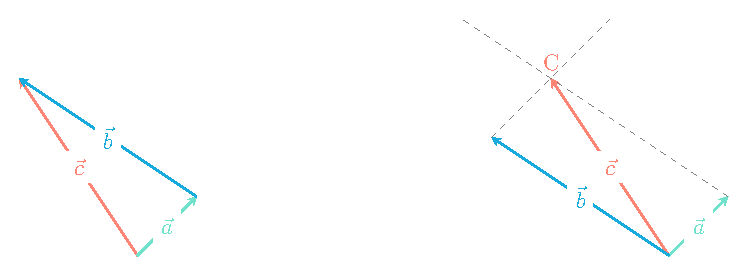
\includegraphics[width=0.8\textwidth]{additonrule}
\caption{三角形法则和平行四边形法则求算矢量}
\end{figure}

三角形法则需要将两个矢量\textbf{头尾相接},而平行四边形法则需要将两个矢量放置在\textbf{同一起点}。但是结果都是一致的。如果做矢量的减法$\vec{a}-\vec{b}$的话,仅需要理解为$\vec{a}+(-\vec{b})$也就是加上和$\vec{b}$相反方向,大小一致的矢量即可。

\subsection*{矢量的正交分解}
\label{subsec:Decomposition of Vectors}
如果建立了坐标系,则可以对任意矢量进行正交分解。示意图可以参考\ref{fig:vectors}。
因此水平方向的分量Component计算公式为$a_x=a\cdot \cos\theta$;
同理,竖直方向的分量计算公式为$a_y=a\cdot \sin \theta$。
反过来也是一样的道理。对两个分量$a_x$和$a_y$进行合成,使用勾股定理,$a=\sqrt{a_x^2+a_y^2}$,$\theta=\arctan ( \frac{a_y}{a_x})$

\subsection*{矢量的坐标表示方案}
承接上一小节,将一个矢量放置在坐标轴当中,并且定义沿着$x$轴正方向的,长度为$1$的矢量为$\vec{i}$,沿着$y$轴正方向的,长度为$1$的矢量为$\vec{j}$,沿着$z$正轴方向的,长度为$1$的矢量为$\vec{k}$。因此\ref{fig:vectors}中,平面矢量$\overrightarrow{OA}$就可以认为是$3\vec{i}+4\vec{j}$的合成结果。那么用更简单的\gls{columnvec}的写法可以表示为$\overrightarrow{OA}=\icol{3\\4}$ 如果是三维矢量的话,$\overrightarrow{OA}=\icol{x\\y\\z}$。

\subsection*{矢量的模(大小)}
\label{subsec:Modulus}
矢量的\gls{modulus}就是指矢量的大小。之前提到过,绘制矢量的图像,该矢量的大小用长度进行表示。现在采用正交分解的方式,矢量的Modulus就可以使用距离公式进行确定:如果是二维平面就是:
\[
	|\overrightarrow{OA}| = \sqrt{x^2+y^2}
\]
如果是三维空间就是:
\[
	|\overrightarrow{OA}| = \sqrt{x^2+y^2+z^2}
\]


\subsection*{任意矢量的单位矢量}
\gls{unitvector}也可以称之为方向矢量,模永远都是$1$。所以,之前提到的$\vec{i}$,$\vec{j}$,$\vec{k}$都可以称之为单位矢量。那么对于任意矢量$\vec{a}$,求算单位矢量$\hat{a}$,仅需要用该矢量$\vec{a}$数乘特定比例$k$,使得单位矢量$\hat{a}$的模为$1$即可。因此该比例$k$就等同于单位矢量的模与初始矢量的模之比,因此
\[
	\hat{a}= \frac{1}{|\vec{a}|} \cdot \vec{a}
\]
\begin{ExampleBox}
求算\ref{fig:vectors}中,平面矢量$\overrightarrow{OP}$的单位矢量
\tcblower
$\overrightarrow{OP}=\icol{3\\4}$\\
$|\overrightarrow{OP}|=\sqrt{3^2+4^2}=5$\\
因此$\overrightarrow{OP}$的单位矢量为:$\frac{1}{5} \cdot \icol{3\\4}=\icol{\frac{3}{5}\\\frac{4}{5}}$
\end{ExampleBox}

\subsection*{矢量的点积}
\label{subsec:Scalar Product}
两个矢量是可以相乘的,分为\gls{dotproduct}和\gls{crossproduct},我们先研究\gls{dotproduct}为:
\[
	\vec{a}\cdot \vec{b}=|\vec{a}||\vec{b}|\cdot \cos{\theta}
\]

\begin{figure}[H]
\centering
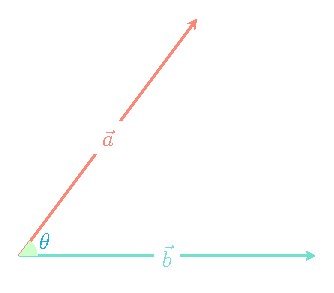
\includegraphics[width=0.8\textwidth]{dotproduct}
\caption{矢量的点积求算}
\end{figure}

两个矢量最终点乘得到结果为\gls{scalar}。因此根据定义,可以得到以下的三个单位矢量互相点乘的计算结果
\begin{align*}
\vec{i}\cdot\vec{i}=|\vec{i}|\cdot|\vec{i}|\cos{0\si{\degree}} =1 \\
\vec{i}\cdot\vec{j}=|\vec{i}|\cdot|\vec{j}|\cos{90\si{\degree}} =0 \\
\vec{i}\cdot\vec{k}=|\vec{i}|\cdot|\vec{k}|\cos{90\si{\degree}} =0 \\
\vec{j}\cdot\vec{i}=|\vec{j}|\cdot|\vec{i}|\cos{90\si{\degree}} =0 \\
\vec{j}\cdot\vec{j}=|\vec{j}|\cdot|\vec{j}|\cos{0\si{\degree}} =1 \\
\vec{j}\cdot\vec{k}=|\vec{j}|\cdot|\vec{k}|\cos{90\si{\degree}} =0 \\
\vec{k}\cdot\vec{i}=|\vec{k}|\cdot|\vec{i}|\cos{90\si{\degree}} =0 \\
\vec{k}\cdot\vec{j}=|\vec{k}|\cdot|\vec{j}|\cos{90\si{\degree}} =0 \\
\vec{k}\cdot\vec{k}=|\vec{k}|\cdot|\vec{k}|\cos{0\si{\degree}} =1 \\
\end{align*}
因此当两个非0矢量\emph{互相垂直的时候}可以推导出这两个矢量的\emph{scalar product等于0}。这两个结论是完全等价的。

因此,如果是用列向量的方式表示两个矢量$\vec{a}=\icol{x_a\\y_a}$ 和 $\vec{b}=\icol{x_b\\y_b}$的话,求算两者的点积会比较简单。其结果为:
\[
	\vec{a}\cdot \vec{b} =\vec{b}\cdot \vec{a} =x_a x_b+y_ay_b
\]

\begin{TaskBox}
利用$\vec{a}=x_a \vec{i}+y_a \vec{j}$和$\vec{b}=x_b \vec{i}+y_b \vec{j}$再相乘尝试证明上述的结果
\end{TaskBox}

如果是三维空间的矢量$\vec{a}=\icol{x_a\\y_a\\z_a}$ 和 $\vec{b}=\icol{x_b\\y_b\\z_b}$,其点乘结果为:
\[
	\vec{a}\cdot \vec{b} = x_ax_b+y_ay_b+z_az_b
\]

\subsection*{矢量的夹角求算}
根据矢量的点乘定义,结合\ref{subsec:Modulus},在给定两个矢量的坐标表示形式的时候,可以利用$cos$值求算这两个矢量的夹角。
\[
	\cos <\vec{a},\vec{b}>=\frac{\vec{a}\cdot\vec{b}}{|\vec{a}|\cdot|\vec{b}|}
\]
在该表达式中,分子是点乘结果,分母是两个矢量的模的乘积,都是可以根据坐标进行求算的,因此经常用于求算两个矢量的夹角。

\begin{ExampleBox}
The direction vector of two lines are $-\mathbf{i}+\mathbf{j}+4\mathbf{k}$ and $2\mathbf{i}+\mathbf{j}-2\mathbf{k}$ respectively. Calculate the acute angle between the directions of the lines.\makebox{}\hfill Adapted from 2017 winter qp33 Q10
\tcblower
记这两个方向矢量分别为$\vec{a}=\icol{-1\\1\\4}$和$\vec{b}=\icol{2\\1\\-2}$。
$\vec{a}\cdot \vec{b}=-1\times2+1\times1+4\times -2=-9$, $|\vec{a}|=\sqrt{(-1)^2+1^2+4^2}=3\sqrt 2$,$|\vec{b}|=\sqrt{2^2+1^2+(-2)^2}=3$
所以两个方向矢量夹角的余弦值为$\frac{-9}{3\sqrt{2}\times 3}=-\frac{\sqrt2}{2}$,方向夹角为$135$\si{\degree}。但是此题求算锐角,因此为$45$\si{\degree}
\end{ExampleBox}
\clearpage


\subsection*{矢量的叉积}
\label{subsec:Cross Product}
两个矢量的\gls{crossproduct}被定义为:

\begin{figure}[H]
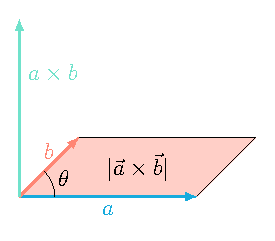
\includegraphics[scale=0.4\textwidth]{crossproduct}
\includegraphics[width=0.4\textwidth]{righthandrule}
\end{figure}

\[
	\vec{a}\times \vec{b}=|\vec{a}||\vec{b}|\cdot \sin{\theta}
\]
两个矢量最终叉乘得到结果为矢量,结果矢量垂直于矢量构成的平面,方向通过右手坐标系进行判断。将$\vec{a}$和$\vec{b}$放置到三维坐标系的$x$和$y$轴中,$z$轴方向就是结果的方向。

因此同理,对基本单位向量的运算得到的结果是:
\begin{flalign*}
\vec{i}\cdot\vec{i}=|\vec{i}|\cdot|\vec{i}|\sin{0\si{\degree}} =\vec{0} \\
\vec{i}\cdot\vec{j}=|\vec{i}|\cdot|\vec{j}|\sin{90\si{\degree}} =\vec{k} \\
\vec{i}\cdot\vec{k}=|\vec{i}|\cdot|\vec{k}|\sin{90\si{\degree}} =-\vec{j} \\

\vec{j}\cdot\vec{i}=|\vec{j}|\cdot|\vec{i}|\sin{90\si{\degree}} =-\vec{k} \\
\vec{j}\cdot\vec{j}=|\vec{j}|\cdot|\vec{j}|\sin{0\si{\degree}} =\vec{0} \\
\vec{j}\cdot\vec{k}=|\vec{j}|\cdot|\vec{k}|\sin{90\si{\degree}} =\vec{i} \\

\vec{k}\cdot\vec{i}=|\vec{k}|\cdot|\vec{i}|\sin{90\si{\degree}} =\vec{j} \\
\vec{k}\cdot\vec{j}=|\vec{k}|\cdot|\vec{j}|\sin{90\si{\degree}} =-\vec{i} \\
\vec{k}\cdot\vec{k}=|\vec{k}|\cdot|\vec{k}|\sin{0\si{\degree}} =\vec{0} \\
\end{flalign*}

这样,我们就定义了两个矢量$\vec{a}=\irow{x_a}{y_a}{z_a}$和$\vec{a}=\irow{x_b}{y_b}{z_b}$叉乘,在坐标系中的运算结果:
\[
	\vec{a}\times\vec{b} =\begin{pmatrix}
      \textbf{i} & \textbf{j} & \textbf{k}\\ 
      x_{a} &   y_{a} & z_{a} \\ 
      x_{b} &   y_{b} & z_{b}
   \end{pmatrix}
\]
\clearpage


\section{空间当中的直线}
利用矢量,现在可以表示空间当中的直线。

\subsection*{位置矢量}
假设$R$是空间当中的任意一点。$A(x,y,z)$通过三个坐标值确定$R$在空间当中的位置。以原点$O$作为起点,以$A$作为终点的矢量就被称之为$A$点的\gls{pos vec}

\subsection*{方向矢量}
从某一个点$A$出发,只需要再给我提供一个方向,就能够绘制一条直线了。该矢量就称之为方向矢量。可以计作$\overrightarrow{AB}$


\subsection*{直线的表示}
因此。如果直线上任何一点$R$的位置矢量,计作$\vec{r}$。必定等于从位置矢量$\vec{a}$出发的矢量+任意倍数的方向矢量进行表示,形式就是:
\[
	\textbf{r} = \textbf{a}+\lambda \textbf{b}
\]
如下图所示:
\begin{figure}[H]
\centering
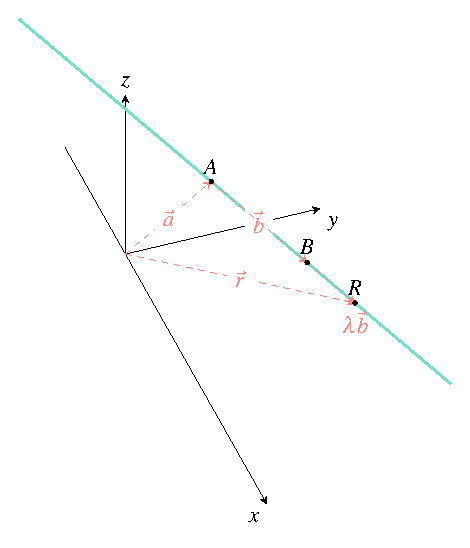
\includegraphics[width=0.8\textwidth]{3Dline}
\label{fig:3Dline}
\caption{三维空间中的直线}
\end{figure}

该表达式本质上在描述直线上任意一点$R$的位置矢量,但是由于满足表达式的所有的点都在在直线$AB$上,因此也被称之为直线的矢量方程。

\begin{TaskBox}
\ref{fig:3Dline}中$A$点的坐标是$(3,2,5)$,$B$点的坐标是$(7,4,4)$。确定直线$AB$的矢量表达式
\tcblower
$\textbf{r} = \icol{3\\2\\5} +\lambda \icol{4\\2\\-1}$是其中的一种结果。实际上可以选择任意直线上的点作为位置矢量,以及方向矢量扩大任意倍数依旧是指向同一方向。因此该直线的表达式有无数多种。
$\textbf{r} = \icol{7\\4\\4} +\lambda \icol{4\\2\\-1}$

$\textbf{r} = \icol{7\\4\\4} +\lambda \icol{-4\\-2\\+1}$
等等都可以
\end{TaskBox}

\subsection*{两条空间内直线的位置关系}
在空间当中,两条直线可能存在的位置关系有:平行,相交,\gls{skew}这三种分类。其中,平行和相交都可以称之为两条直线共面coplanar。为了研究方便,我们规定这两条直线被记做$l_1$和$l_2$,其矢量表示法分别是$\mathbf{r}=\mathbf{a_1}+\lambda \mathbf{b_1}$和$\mathbf{r}=\mathbf{a_2}+\mu \mathbf{b_2}$

\subsubsection*{平行}
当两条直线方向相同时。且没有重合点的时候,两条直线就是垂直的。因此仅需要满足:
\begin{align*}
	\mathbf{b_1} &= c \mathbf{b_2} \qquad c \text{ is a constant}\\
	\mathbf{a_1} &\neq \mathbf{a_2}+\mu \mathbf{b_2}
\end{align*}

\subsubsection*{相交和异面}
空间中直线的相交和异面的关系是较难直接从二维图像当中看出来的。如下图所示:
\begin{figure}[H]
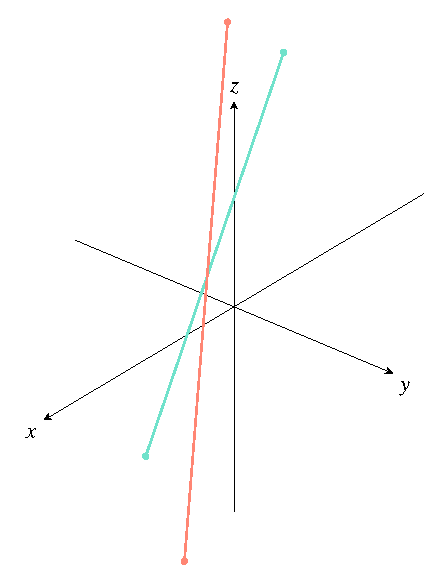
\includegraphics[width=0.4\textwidth]{skew1}
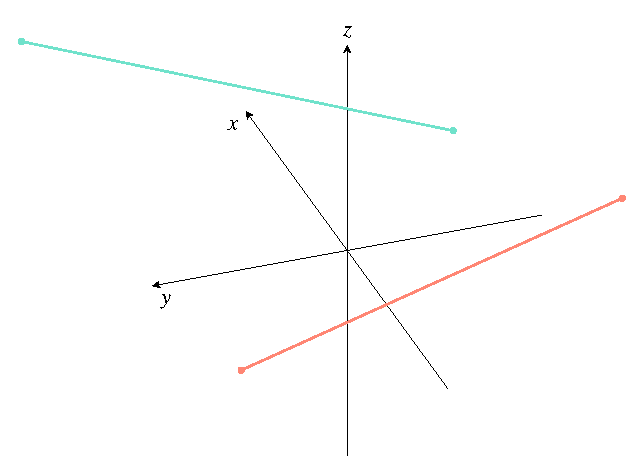
\includegraphics[width=0.6\textwidth]{skew2}
\end{figure}
所以,需要利用直线的矢量形式,如果存在一个点$R$既在直线$l_1$上,也在$l_2$上的话。那么就意味着$R$点坐标能够同时满足两条直线的表达式。但是要注意,方向矢量前的系数可以是不一致的。因此联立求解方程。
\[
	\mathbf{a_1}+\lambda \mathbf{b_1}=\mathbf{a_2}+\mu \mathbf{b_2}
\]

\begin{SummBox}
该方程只需要求解$\lambda$和$\mu$这两个未知数即可,但是却有三个方程(交点的三个坐标),因此,利用两个进行求解的时候,求算出$\lambda$和$\mu$的值之后,还需要带入到第三个方程中进行检验,如果能够成立,则证明两条线确实\textbf{相交};如果检验之后不成立,则证明两条线实际上是\textbf{异面}的关系
\end{SummBox}

\subsection*{点到直线的垂线}
这类型的题目没有在考纲当中没有明确写出来,但是考试还是要考察的,可恶!

不过基本思路并不难。重点就是找到直线上可以作为\textbf{垂足}的点。一旦垂足被确定了,就可以去利用距离公式求算该点到垂足的距离,借此作为点到直线的距离。

因此整体的思路就是利用直线的矢量方程表示垂足,利用垂足和方向矢量的垂直关系,也就是两个矢量的\textbf{点积为0}去求算参数$\lambda$。进而确定垂足的坐标。

\begin{ExampleBox}
With respect to the origin $O$, the vertices of a triangle $ABC$ have position vectors.
\[
	\overrightarrow{OA}= 2\mathbf{i}+5\mathbf{k}, \quad \overrightarrow{OB}= 3\mathbf{i}+2\mathbf{k}+3\mathbf{k}, \quad \overrightarrow{OC}= \mathbf{i}+\mathbf{j}+\mathbf{k} 
\]
Find the exact length of the perpendicular from $O$ to the line through $B$ and $C$.

\tcblower
首先,找出$BC$的直线表达式,利用位置矢量$\overrightarrow{OB}=\icol{3\\2\\3}$和方向矢量$\overrightarrow{CB}=\icol{2\\1\\2}$,因此直线$BC$的方程就是:
\[\mathbf{r}=\icol{3\\2\\3}+\lambda\cdot\icol{-2\\-1\\-2}\]
接下来第二步就是,寻找垂足$D$点的坐标。利用$\overrightarrow{OD}\cdot \overrightarrow{BC}=0$得到如下的表达式:
\[
	\icol{3-2\lambda\\2-\lambda\\3-2\lambda}\cdot\icol{-2\\-1\\-2}=0
\]
化简得到关于参数$\lambda$的方程:
\[
	(3-2\lambda)\cdot(-2)+(2-\lambda)\cdot(-1)+(3-2\lambda)\cdot(-2)=0
\]
求解之后得到$\lambda = \frac{14}{9}$。将其带入表达式当中获得垂足的坐标为$R(-\frac{1}{9},\frac{4}{9},-\frac{1}{9})$
所以$O$到直线的距离就是$OR=\sqrt{(-\frac{1}{9})^2+(\frac{4}{9})^2+(-\frac{1}{9})^2}=\frac{\sqrt2}{3}$。
\end{ExampleBox}
可以点击\href{https://www.geogebra.org/m/n7cqaqtd}{geogebra链接}进行AR观察





